% Generated by analyze_t8.js - paste before \end{document}
\subsection{T8 -- Effect of supply-chain complexity}
Executed on 2026-10-21 (11:37--12:15 CEST), sequential submission.
Part A: one EXTRACTION transformation with $n \in \{1, 5, 10, 25, 50, 100\}$ input lots (3 runs $\times$ 8
iterations, 1 warm-up iteration per run excluded), followed by packaging, binding, 5 UID verifications,
certificate query and consumption. Part B: chains of $d \in \{1, 5, 10, 20\}$ successive DRYING transformations
(5 chains per depth, 1 warm-up chain excluded), followed by the same steps. Input lots were prepared in parallel
and are not part of the measurements. 816 measured transactions; 0 failures;
0 retries of a measured step because the previous step had not yet been committed on the second peer.

\begin{table}[H]
\centering\small
\caption{T8-A: chaincode execution ($L^{\mathrm{end}}$, mean $\pm$ SD, ms), UID verification latency and certificate size as
a function of the number of input lots.}
\label{tab:t8a}
\setlength{\tabcolsep}{3.5pt}
\begin{tabular}{rrrrrrr}
\toprule
$n$ & Samples & Transf. & Packaging & Binding & Verif. & Cert.\ (B) \\
\midrule
1 & 24 & 29.0 $\pm$ 3.4 & 17.0 & 29.7 $\pm$ 5.0 & 11.5 & 1124 \\
5 & 24 & 39.9 $\pm$ 4.2 & 17.1 & 28.8 $\pm$ 9.7 & 9.8 & 1236 \\
10 & 24 & 55.1 $\pm$ 6.9 & 15.4 & 26.9 $\pm$ 2.9 & 9.3 & 1373 \\
25 & 24 & 93.1 $\pm$ 10.4 & 16.4 & 28.1 $\pm$ 9.0 & 8.9 & 1780 \\
50 & 24 & 149.1 $\pm$ 11.1 & 14.9 & 28.0 $\pm$ 2.4 & 9.4 & 2457 \\
100 & 24 & 257.0 $\pm$ 18.2 & 13.0 & 27.2 $\pm$ 5.0 & 8.5 & 3809 \\
\bottomrule
\end{tabular}
\end{table}

\begin{table}[H]
\centering\small
\caption{T8-B: chaincode execution ($L^{\mathrm{end}}$, ms) and UID verification latency as a function of the chain depth.}
\label{tab:t8b}
\setlength{\tabcolsep}{3.5pt}
\begin{tabular}{rrrrrrr}
\toprule
$d$ & Chains & Transf.\ (mean) & Last transf. & Binding & Verif. & Cert.\ (B) \\
\midrule
1 & 5 & 24.1 & 24.1 & 27.9 & 8.0 & 1135 \\
5 & 5 & 19.3 & 18.5 & 23.4 & 8.0 & 1142 \\
10 & 5 & 18.0 & 18.6 & 26.3 & 8.5 & 1142 \\
20 & 5 & 18.2 & 19.3 & 23.5 & 9.5 & 1142 \\
\bottomrule
\end{tabular}
\end{table}

\begin{figure}[H]
\centering
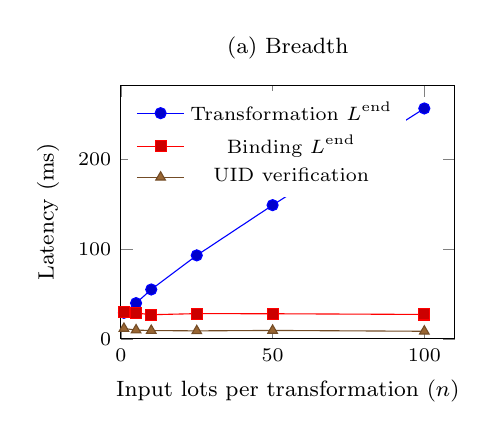
\begin{tikzpicture}
\begin{axis}[width=0.48\linewidth, height=4.8cm, xlabel={Input lots per transformation ($n$)}, ylabel={Latency (ms)},
  xmin=0, ymin=0, tick label style={font=\scriptsize}, label style={font=\footnotesize},
  legend style={font=\scriptsize, at={(0.02,0.98)}, anchor=north west, draw=none}, title={(a) Breadth}, title style={font=\footnotesize}]
\addplot+[mark=*] coordinates {(1,29.00) (5,39.85) (10,55.07) (25,93.12) (50,149.15) (100,257.02)};
\addlegendentry{Transformation $L^{\mathrm{end}}$}
\addplot+[mark=square*] coordinates {(1,29.66) (5,28.82) (10,26.91) (25,28.13) (50,27.99) (100,27.22)};
\addlegendentry{Binding $L^{\mathrm{end}}$}
\addplot+[mark=triangle*] coordinates {(1,11.52) (5,9.80) (10,9.26) (25,8.89) (50,9.37) (100,8.45)};
\addlegendentry{UID verification}
\end{axis}
\end{tikzpicture}\hfill
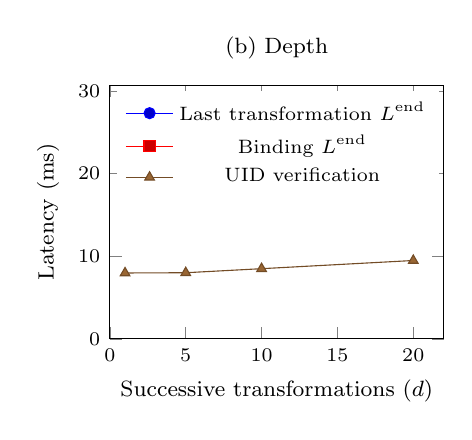
\begin{tikzpicture}
\begin{axis}[width=0.48\linewidth, height=4.8cm, xlabel={Successive transformations ($d$)}, ylabel={Latency (ms)},
  xmin=0, ymin=0, tick label style={font=\scriptsize}, label style={font=\footnotesize},
  legend style={font=\scriptsize, at={(0.02,0.98)}, anchor=north west, draw=none}, title={(b) Depth}, title style={font=\footnotesize}]
\addplot+[mark=*] coordinates {(1,24.08) (5,18.50) (10,18.56) (20,19.31)};
\addlegendentry{Last transformation $L^{\mathrm{end}}$}
\addplot+[mark=square*] coordinates {(1,27.88) (5,23.41) (10,26.34) (20,23.51)};
\addlegendentry{Binding $L^{\mathrm{end}}$}
\addplot+[mark=triangle*] coordinates {(1,7.97) (5,8.00) (10,8.49) (20,9.48)};
\addlegendentry{UID verification}
\end{axis}
\end{tikzpicture}
\caption{Cost as a function of supply-chain complexity (sequential submission, mean values): (a) one transformation with
$n$ input lots; (b) a chain of $d$ successive transformations before packaging and binding.}
\label{fig:eval-complexity}
\end{figure}

\paragraph{Observations.}
\begin{itemize}
  \item \textbf{Breadth.} Linear fits: transformation 30.94 + 2.29\,$n$\,ms ($R^2 = 1.00$); binding
        28.58 + -0.01\,$n$\,ms ($R^2 = 0.29$); verification 10.15 + -0.02\,$n$\,ms
        ($R^2 = 0.44$); certificate size 1101 + 27.1\,$n$ bytes.
  \item \textbf{Depth.} Slopes per additional upstream transformation: binding -0.16\,ms, verification
        0.08\,ms, certificate size 0.3 bytes; the verification cost does not depend on the depth of
        the chain because only the immediate transformation is hashed into the certificate.
  \item \textbf{Scope.} Inputs within a transformation are processed by a single chaincode invocation, whose payload limit
        (16\,KB) and the implementation limit of 100 input lots bound the breadth that can be expressed in one transaction.
\end{itemize}
